\chapter{Mini-Project A}
\label{sec:ProjA}
This project examines ELO5.2, which requires the student to develop a representative embedded system. It requires hardware/software interfacing, so an ADC is sampled by software, and processing operations are applied to read the data. 

\section{Project Requirements}
The Project is split into Milestones in order to help you plan time and ensure you aren't overburdened with work a few days before the final deadline. Dates for submission will be put on Vula. The milestones are as follows:
\begin{enumerate}
    \renewcommand{\theenumi}{\Alph{enumi}}
    \item Planning and System Design\\
    For this milestone we expect to see the following:
    \begin{itemize}
        \item A Gantt Chart indicating your planned activities with the project
        \item A circuit diagram for the system
        \item A choice on how you plan to approach the project (e.g. Spiral, waterfall, etc.) as well as a justification as why
        \item A flowchart detailing how the system operates
    \end{itemize}
    \item Progress update\\
    For this milestone we expect to see the following:
    \begin{itemize}
        \item A review on your Gantt chart to see if you've been meeting deadlines
        \item A review on your design plan, noting any changes
        \item 3 things you've implemented since the previous milestone submission, such as work on the report or implementation, along with evidence of what you've implemented.
    \end{itemize}
    \item Demo\\
    For this milestone you will create a YouTube video. Details on the requirements of the Video are found in the marking guides. 
    \item Code and Report\\
    The final hand in will be the report and your code submission. Details on these can be found in the marking guides.
\end{enumerate}

\section{Outcomes}
In addition to creating a working system, you will learn about the following in this project:
\begin{itemize}
    \item Technical outcomes
    \begin{itemize}
        \item ADC - \href{https://cdn-shop.adafruit.com/datasheets/MCP3008.pdf}{MCP3008}
        \item Temperature sensor - \href{http://ww1.microchip.com/downloads/en/devicedoc/20001942g.pdf}{MCP9700A}
        \item IOT - \href{https://blynk.io/}{Blynk}
    \end{itemize}
    \item Other outcomes
    \begin{itemize}
        \item Team Work
        \item Design methodologies, such as the Waterfall, Spiral and V Models.
        \item Planning and time management
    \end{itemize}
    
    
\end{itemize}

\section{Deliverables}
At the end of this project, you must:
\begin{itemize}
    \item Submit all milestones
    \item Demonstrate your working implementation to a tutor through a formal presentation. This will take the form of a YouTube video no longer than 8 minutes long. See \ref{tbl:DemoValidation} for details on the demonstration.
    \item Submit your report to Vula, in the format shown in Table \ref{tbl:ProjAMarks}
    \item For information on the marks and what sections to cover, refer to the marking guide in Section \ref{sec:ProjAMarks}
\end{itemize}

% \section{Hardware Required}
% \begin{tabular}{ll}
% \begin{tabular}[c]{@{}l@{}}
% \tabitem All hardware from previous pracs\\ 
% \tabitem LDR\\
% \end{tabular} 
% &\begin{tabular}[c]{@{}l@{}}
% \tabitem ADC\\ 
% \tabitem Temperature Sensor\\ 
% \\
% \end{tabular} 
% \end{tabular}
\section{System Overview}
Figure \ref{fig:SystemOverview} shows the system overview for the mini-project.
\begin{figure}[H]
\centering
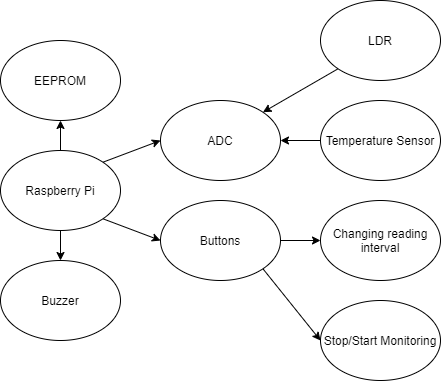
\includegraphics[width=0.6\columnwidth]{Figures/SystemOverview}
\caption{Components of the Mini-Project}
\label{fig:SystemOverview}
\end{figure}




\section{Hardware requirements}
You will need to build your designed circuit on a breadboard and demonstrate it in the video you create.

\section{Software requirements}
You need to do the following:
\begin{itemize}
    \item Set up the EEPROM. 
    \item Create a thread for reading from the ADC. The value read from the temperature sensor needs to be converted to degrees Celsius. See the datasheet (linked above) for the formula.
    \item Create interrupts for all the button functionality (don't forget to debounce your inputs)
    \item Create an output signal to trigger the buzzer.
    \item In the main() loop, print values to the screen as described in Section \ref{sec:ProjDescription}
\end{itemize}

\section{Description}
\label{sec:ProjDescription}
\begin{itemize}
    \item By default, the system continuously monitors the sensors every 5s using this format:
    \begin{table}[H]
    \centering
    \begin{tabular}{|l|l|l|l|l|l|}
    \hline
    Time     & Sys Timer & Light  & Temp & Light &  Buzzer  \\ \hline
    10:17:15 & 00:00:00  & 0.5 V  & 25 C & 595   & *        \\ \hline
    10:17:20 & 00:00:05  & 1.5 V  & 25 C & 595   &          \\ \hline
    10:17:25 & 00:00:10  & 1.7 V  & 25 C & 595   &          \\ \hline
    10:17:30 & 00:00:15  & 2.2 V  & 25 C & 782   &          \\ \hline
    10:17:35 & 00:00:20  & 3.3 V  & 25 C & 998   &          \\ \hline
    10:17:35 & 00:00:20  & 3.3 V  & 25 C & 998   & *        \\ \hline
    \end{tabular}
    \end{table}
    \item The stop switch stops or starts the monitoring of the sensors. The system timer is not affected by this functionality. The screen must also be cleared when logging is stopped, and a message printed to display the information to the user.
 
\end{itemize}

\section{Marking Guide}
\label{sec:ProjAMarks}
\begin{longtable}[c]{|l|l|l|}
\caption{Project A marking Guide}
\label{tbl:ProjAMarks}
\\\hline
\textbf{Heading} & \textbf{Report} & \textbf{Demo} \\ \hline
\endfirsthead
%
\endhead
%
Introduction & \begin{tabular}[c]{@{}l@{}}Provide a short introduction ($\sim \frac{1}{2}$ page)\\ to your project explaining your main\\ design choices and how the report has\\ been structured \textbf{{[}15 marks{]}}\end{tabular} & \begin{tabular}[c]{@{}l@{}}Introduce yourselves and\\ your project. \textbf{{[}8 marks{]}}\end{tabular} \\ \hline
Requirements & \begin{tabular}[c]{@{}l@{}}The requirements section should\\ provide a refined UML Use Case\\ diagram of the system, according to\\ your implementation, and any\\ accompanying text that is needed to\\ clarify the requirements.\\ Highlight any departures or additions\\ that you may have made compared to\\ the original project description given in\\ this document. \textbf{{[}15 marks{]}}\end{tabular} & \begin{tabular}[c]{@{}l@{}}Have an (at least draft)\\ UML Use Case to show\\ the tutor. Show this\\ briefly, indicating any\\ departures/additions.\\ \textbf{{[}6 marks{]}}\end{tabular} \\ \hline
\begin{tabular}[c]{@{}l@{}}Specification \\ and Design\end{tabular} & \begin{tabular}[c]{@{}l@{}}This section should provide a UML\\ State Chart describing the main\\ operation. Add a UML class or\\ deployment diagram (or other suitable\\ diagram) to indicate the structuring of\\ your implementation (e.g. code\\ modules/classes you may be using).\\ You don’t need to provide fine detail of\\ the system, the diagram(s) can be e.g.\\ at the level of functions. You should\\also include a circuit diagram \textbf{{[}20 marks{]}}\end{tabular} & \begin{tabular}[c]{@{}l@{}}Briefly show your design,\\ you need not show more\\ than one rough diagram\\ (e.g. draft state chart) to\\ the tutor. \textbf{{[}10 marks{]}}\end{tabular} \\ \hline
Implementation & \begin{tabular}[c]{@{}l@{}}This section should give some snippets\\ of important code and explanations for\\ this (or referring to particular\\ functions in code files). The point here\\ is elaborating any parts of the State\\ Chart that are not so straightforward\\ to turn into code. \textbf{{[}20 marks{]}}\end{tabular} & \begin{tabular}[c]{@{}l@{}}You should have a code\\ file open already (e.g.\\ where the main function\\ is) before you start the\\ demo. Briefly confirm to\\ the tutor that this is part\\ of the program that will be\\ demoed. \textbf{{[}6 marks{]}}\end{tabular} \\ \hline
\begin{tabular}[c]{@{}l@{}}Validation and\\ Performance\end{tabular} & \begin{tabular}[c]{@{}l@{}}Provide at least a paragraph or two\\ explaining the performance of the\\ system. A snapshot could be included\\ and you could show test cases where\\ you have tested that the system works\\ reliably (e.g. using a powersupply to set \\ the value given to the ADC). \textbf{{[}20}\\ \textbf{marks{]}}\end{tabular} & \begin{tabular}[c]{@{}l@{}}This is a main aspect of\\ the demonstration.\\ See Validation Check\\ Sheet in Section \ref{sec:ProjAValidation}.\\ \textbf{{[}30 marks{]}}\end{tabular} \\ \hline
Conclusion & \begin{tabular}[c]{@{}l@{}}Give a summary of the extent that the\\ system was found to be successful.\\ Discuss if you think that a system\\ working in this way might be\\ considered a potentially useful product.\\ \textbf{{[}10 marks{]}}\end{tabular} & \begin{tabular}[c]{@{}l@{}}End you demo with a\\ short conclusion, reflect\\ on the activity. \textbf{{[}10 marks{]}}\end{tabular} \\ \hline
References & Provide a few references if relevant. &  \\ \hline
Total & 100 &  \\ \hline
\end{longtable}

\section{Project A Demo Validation Sheet}

\label{sec:ProjAValidation}
\begin{table}[H]
\caption{The Mark sheet for the tech demo aspect of your project}
\label{tbl:DemoValidation}
\centering
\resizebox{\textwidth}{!}{%
\begin{tabular}{|l|l|l|r|c|}
\hline
% \multicolumn{3}{|l|}{{\ul \textbf{Project Validation Sheet}}}  & \multicolumn{2}{l|}{\begin{tabular}[c]{@{}l@{}}\textbf{Marked by:} \\ \\\end{tabular}} \\ \hline
% \multicolumn{7}{|l|}{\begin{tabular}[c]{@{}l@{}}\textbf{Student Numbers:} \\ \\ \\\end{tabular}} \\ \hline
\textbf{Category} & \textbf{Item} & \textbf{Description} & \multicolumn{1}{c|}{Max Mark} & \begin{tabular}[c]{@{}c@{}}Attempt\\ 1\end{tabular} \\ \hline 
\textbf{Blynk} & \begin{tabular}[c]{@{}l@{}}Connected \\ and responds\end{tabular} & \begin{tabular}[c]{@{}l@{}}Blynk should connect to\\ the pi (2) and respond to \\ changes on the pi (5 - ldr, \\ temp, buzzer, start/stop \\ log, change interval)\end{tabular} & 7 &    \\ \hline
\textbf{} & Design & \begin{tabular}[c]{@{}l@{}}All features of the should\\ be reflected in the widgets\\ used in Blynk\end{tabular} & 5 &  \\ \hline
 &  & \begin{tabular}[c]{@{}l@{}}The use of widgets should\\ be aesthetically pleasing as\\ well as intuitive (use of labels,\\ placement of widgets)\end{tabular} & 2 &  \\ \hline
ADC & Temperature & \begin{tabular}[c]{@{}l@{}}Temperature reported on is\\ accurate and responds to \\ input (warming up when \\ sensor is held, etc)\end{tabular} & 3 &  \\ \hline
%  & Potentiometer & \begin{tabular}[c]{@{}l@{}}Responds to changes input, \\ reading displayed is between\\ 0 and 3.3V\end{tabular} & 2 &  &  &  \\ \hline
 & Light sensor & Voltage divider & 2 & \begin{tabular}[c]{@{}l@{}} \\ \\\end{tabular}  \\ \hline
 &  & \begin{tabular}[c]{@{}l@{}}Reports a value between\\ 0 and 1023\end{tabular} & 2 &  \\ \hline
\begin{tabular}[c]{@{}l@{}}Buttons/\\ Logging\end{tabular} & Implementation & \begin{tabular}[c]{@{}l@{}}Uses interrupts (1 ea) and \\ debouncing (1 ea)\end{tabular} & 4 &   \\ \hline
 & Interval Reading & Changes between 5, 10 and 15s & 3 & \begin{tabular}[c]{@{}l@{}} \\ \\\end{tabular} \\ \hline
 & Reset SysTime & Resets system time to 0 & 1 & \begin{tabular}[c]{@{}l@{}} \\ \\\end{tabular} \\ \hline
 & \begin{tabular}[c]{@{}l@{}}Stop/Start \\ logging\end{tabular} & \begin{tabular}[c]{@{}l@{}}Pauses the print out to \\ system console, but timer \\ continues increasing\end{tabular} & 1 &    \\ \hline
Mark &  &  & 30 & \begin{tabular}[c]{@{}l@{}} \\ \\\end{tabular} \\ \hline
\end{tabular}%
}
\end{table}